\setmodule{9}

%BEGIN_FOLD % ====>>_____ Занятие 1 _____<<====
\begin{class}[number=1]
	\begin{listofex}
		\item По озеру плавала яхта. Расстояние \(s\) (в километрах), на которое удалялась яхта от базы, менялось с течением времени движения (в минутах). Изменение \(s\) в зависимости от t показано на рисунке. 
		\begin{tasks}
			\task На каком расстоянии от базы находилась яхта через \(20\) минут?
			\task На каком расстоянии от базы находилась яхта через \(1\) час \(20\) минут?
			\task На каком расстоянии от базы находилась яхта через \(2\) часа \(30\) минут?
			\task Какова область определения рассматриваемой функции?
		\end{tasks}
		\begin{minipage}[t]{\linewidth}
			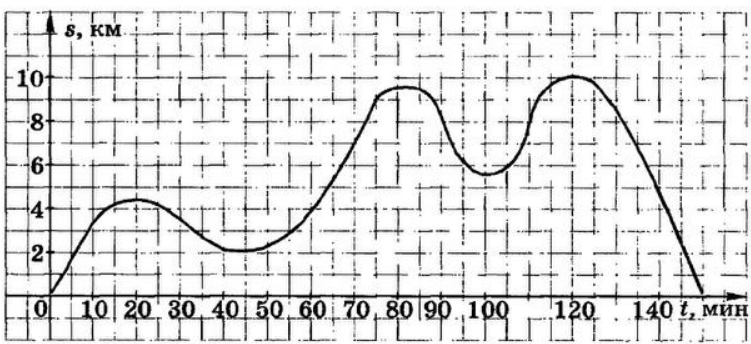
\includegraphics[align=t, width=\linewidth]{\picpath/../../bank/graphs/graph_gleb/7/G71M9L1-1}
		\end{minipage}
		\item Функция задана формулой \(y=\dfrac{ 12 }{ x }\). В таблице указаны некоторые значения аргумента. Заполните таблицу, вычислив соответствующие значения функции:
		\begin{minipage}[t]{\linewidth}
			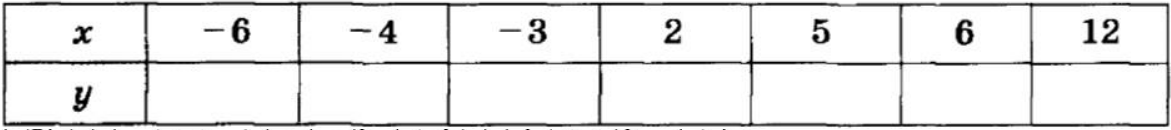
\includegraphics[align=t, width=\linewidth]{\picpath/../../bank/graphs/graph_gleb/7/G71M9L1-2}
		\end{minipage}
		\item Функция задана формулой \(y=\dfrac{ 2}{ 3 }x\). Заполните таблицу:
		\begin{minipage}[t]{\linewidth}
			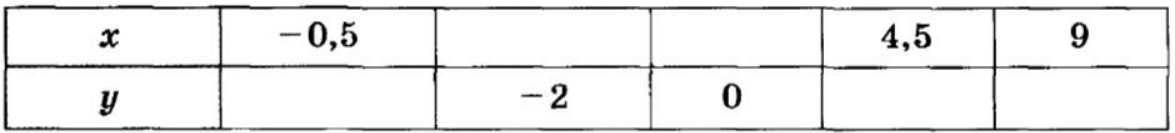
\includegraphics[align=t, width=\linewidth]{\picpath/../../bank/graphs/graph_gleb/7/G71M9L1-3}
		\end{minipage}
		%255-257
		\item На рисунке представлены графики линейных функций. Для каждой функции определите знаки \(k\) и \(b\). \\
		\begin{minipage}[t]{0.45\linewidth}
			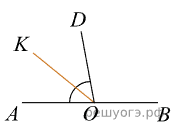
\includegraphics[align=t, width=\linewidth]{\picpath/../../bank/graphs/graph_gleb/7/1}
		\end{minipage}
		\gapwidth
		\begin{minipage}[t]{0.45\linewidth}
			\includegraphics[align=t, width=\linewidth]{\picpath/../../bank/graphs/graph_gleb/7/2}
		\end{minipage}
		\item 
		\begin{minipage}[t]{\bodywidth}
			Сопоставьте каждому уравнению его график:
			\begin{tasks}
				\task \( y=-2x+5 \)
				\task \( y=-\dfrac{ 2 }{ 3 }x+5 \)
				\task \( y=-6x+5 \)
			\end{tasks}
		\end{minipage}
		\gapwidth
		\begin{minipage}[t]{\picwidth}
			\includegraphics[align=t, width=\linewidth]{\picpath/../../bank/graphs/graph_gleb/7/3}
		\end{minipage}
		\item 
		\begin{minipage}[t]{\bodywidth}
			Сопоставьте каждому уравнению его график:
			\begin{tasks}
				\task \( y=-2x+5 \)
				\task \( y=-2x \)
				\task \( y=-2x-5 \)
			\end{tasks}
		\end{minipage}
		\gapwidth
		\begin{minipage}[t]{\picwidth}
			\includegraphics[align=t, width=\linewidth]{\picpath/../../bank/graphs/graph_gleb/7/4}
		\end{minipage}
		%260 а-г
		\item Не выполняя построения, определите, в каких четвертях лежит график
		функции:
		\begin{tasks}(2)
			\task \( y=9x-6 \)
			\task \( y=-8 \)
			\task \( y=-5x \)
			\task \( y=-2x+7 \)
		\end{tasks}
		
	\end{listofex}
\end{class}
%END_FOLD

%BEGIN_FOLD % ====>>_____ Занятие 2 _____<<====
\begin{class}[number=2]
	\begin{listofex}
		%258
		\item Сопоставьте каждой прямой на рисунке уравнение, которым она может быть задана:
		\begin{tasks}(2)
			\task \( y=-8 \)
			\task \( y=2x \)
			\task \( y=-7x+3 \)
			\task \( y=\dfrac{ 2 }{3  }x-1 \)
			\task \( y=0,5 \)
			\task \( y=100x+\dfrac{ 2 }{ 11 } \)
			\task \( y=-3,6x-2 \)
			\task \( y=-9x \)
		\end{tasks}
		\begin{minipage}[t]{\linewidth}
			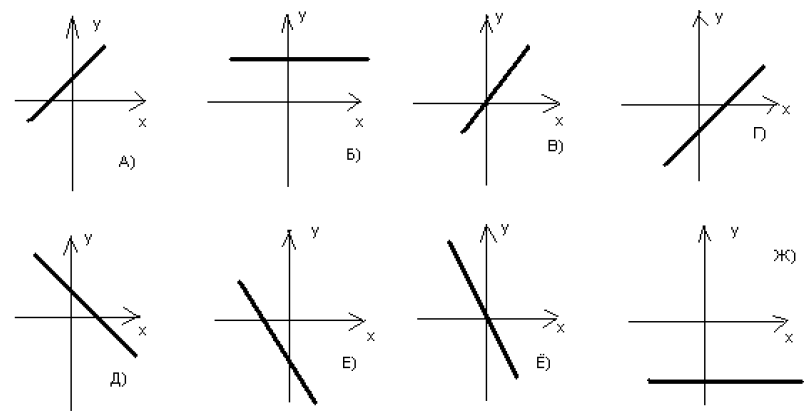
\includegraphics[align=t, width=\linewidth]{\picpath/../../bank/graphs/graph_gleb/7/G71M9L2-1}
		\end{minipage}
		%261 а-е
		\item Не выполняя построения, найдите координаты точек пересечения графиков функций:
		\begin{tasks}
			\task \( y=5x-3 \) и \( y=-x+15 \)
			\task \( y=7-x \) и \( y=2x-2 \)
			\task \( y=-7x-1 \) и \( y=11x-2 \)
			\task \( y=8x-3 \) и \( y=7x+12 \)
			\task \( y=\dfrac{ 2 }{ 3 }x+4 \) и \( y=x+1 \)
			\task \( y=-0,6x-1 \) и \( y=2x+1 \)
		\end{tasks}
		%260 Д-Ё
		\item Не выполняя построения, определите, в каких четвертях лежит график функции:
		\begin{tasks}(2)
			\task \( y=-x-13 \)
			\task \( y=1 \)
			\task \( y=6x+1 \)
			\task \( y=5x \)
		\end{tasks}
		\item Задайте формулой линейную функцию, график которой параллелен прямой \(y=-4x+11\) и проходит через точку \(A(- 3; 5)\).
		\item Задайте формулой линейную функцию, график которой параллелен прямой \(y=6+2x\) и проходит через точку \(A(7; -12)\).
		\item Задайте формулой линейную функцию, график которой параллелен прямой \(y=-4-x\) и проходит через точку \(A(12; -8)\).
	\end{listofex}
\end{class}
%END_FOLD

%BEGIN_FOLD % ====>>_ Домашняя работа 1 _<<====
\begin{homework}[number=1]
	\begin{listofex}
		\item 
		\begin{minipage}[t]{0.4\linewidth}
		Сопоставьте каждой прямой на рисунке уравнение, которым она может быть задана:
		\begin{tasks}(1)
			\task \( y=0,5 x+4 \)
			\task \( y=5x + 8 \)
			\task \( y=-x-2 \)
			\task \( y=-2x+5 \)
		\end{tasks}
	\end{minipage}
		\begin{minipage}[t]{0.55\linewidth}
			\includegraphics[align=t, width=\linewidth]{\picpath/../../bank/graphs/graph_gleb/7/G71M9H1-1}
		\end{minipage}
		%\item Постройте на координатной плоскости функции:
		%\begin{tasks}(4)
		%	\task \( y=5x-2 \)
		%	\task \( y=-x+3 \)
		%	\task \( y=-2x \)
		%	\task \( y=\dfrac{ x }{ 4 }+1 \)
		%\end{tasks}
		
		%261 VES
		\item Не выполняя построения, найдите координаты точек пересечения графиков функций:
		\begin{tasks}
			\task \( y=13x +5 \) и \(y=12,3x-4\)
			\task \( y=0,7x-3 \) и \(y=-0,2x+6\)
			\task \( y=-5x-7 \) и \( y=4x-0,2 \)
			\task \( y=5,2-6x \) и \( y=x-0,7 \)
		\end{tasks}
		\item Решите системы уравнений:
		\begin{tasks}(3)
			\task \( \begin{cases} y-x=8 \\ 2x+y=11 \end{cases} \)
			\task \( \begin{cases} 3x+4y = 12 \\ y+7=x \end{cases} \)
			\task \( \begin{cases} y-2x=5,5 \\ x=5-y \end{cases} \)
		\end{tasks}
	\end{listofex}
\end{homework}
%END_FOLD

%BEGIN_FOLD % ====>>_____ Занятие 3 _____<<====
\begin{class}[number=3]
	\begin{listofex}
		%c188
		\item Решите системы уравнений:
		\begin{tasks}(2)
			\task \( \begin{cases} 2x-3y+1=0 \\ x+2y+4=0 \end{cases} \)
			\task \( \begin{cases} x-y=-1 \\ 2x-2y+3=0 \end{cases} \)
			\task \( \begin{cases} 2x+y=-2 \\ 6x+3y=-6 \end{cases} \)
			\task \( \begin{cases} 3x+4y-1=0 \\ 2x+5y=5 \end{cases} \)
			\task \( \begin{cases} 2x+2y=7 \\ 4x-3y=5 \end{cases} \)
			\task \( \begin{cases} -5x=3-y \\ x-2=3-y \end{cases} \)
		\end{tasks}
		%260 Д-Ё
		\item Не выполняя построения, определите, в каких четвертях лежит график функции:
		\begin{tasks}(2)
			\task \( y=-x-13 \)
			\task \( y=1 \)
			\task \( y=6x+1 \)
			\task \( y=5x \)
		\end{tasks}
		\item Задайте формулой линейную функцию, график которой параллелен прямой \(y=-4x+11\) и проходит через точку \(A(- 3; 5)\).
		\item Задайте формулой линейную функцию, график которой параллелен прямой \(y=6+2x\) и проходит через точку \(A(7; -12)\).
		\item Задайте формулой линейную функцию, график которой параллелен прямой \(y=-4-x\) и проходит через точку \(A(12; -8)\).
		%\item Решите системы уравнений:
		%\begin{tasks}
		%	\task \( \begin{cases}  \\  \end{cases} \)
		%	\task \( \begin{cases}  \\  \end{cases} \)
		%	\task \( \begin{cases}  \\  \end{cases} \)
		%	\task \( \begin{cases}  \\  \end{cases} \)
		%\end{tasks}
	\end{listofex}
\end{class}
%END_FOLD

%BEGIN_FOLD % ====>>_____ Занятие 4 _____<<====
\begin{class}[number=4]
	\begin{listofex}
		%RESHU OGE 322008 339091 341325
		\item Установите соответствие между графиками функций и формулами, которые их задают.
		\begin{minipage}[t]{\linewidth}
			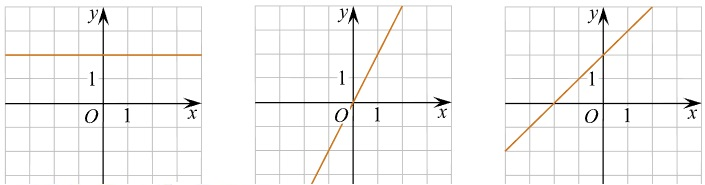
\includegraphics[align=t, width=\linewidth]{\picpath/G71M9L4-1}
		\end{minipage}
		\\
		\\
		\begin{minipage}[t]{\linewidth}
			\begin{tasks}(4)
				\task \( y=2x \)
				\task \( y=-2x \)
				\task \( y=x+2 \)
				\task \( y=2 \)
			\end{tasks}
		\end{minipage}
		
		\item 
		\begin{minipage}[t]{0.35\linewidth}
			Установите соответствие между функциями и их графиками.
			\begin{tasks}(1)
				\task \( y=-2x+4 \)
				\task \( y=2x-4 \)
				\task \( y=2x+4 \)
			\end{tasks}
		\end{minipage}
		\begin{minipage}[t]{0.6\linewidth}
			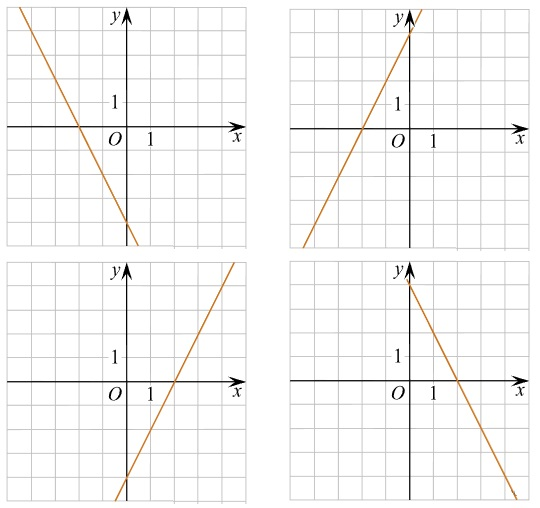
\includegraphics[align=t, width=\linewidth]{\picpath/G71M9L4-2}
		\end{minipage}
		
		\item На рисунке изображены графики функций вида \(y = kx + b\). Установите соответствие между графиками функций и знаками коэффициентов \(k\) и \(b\).
		\begin{minipage}[t]{\linewidth}
			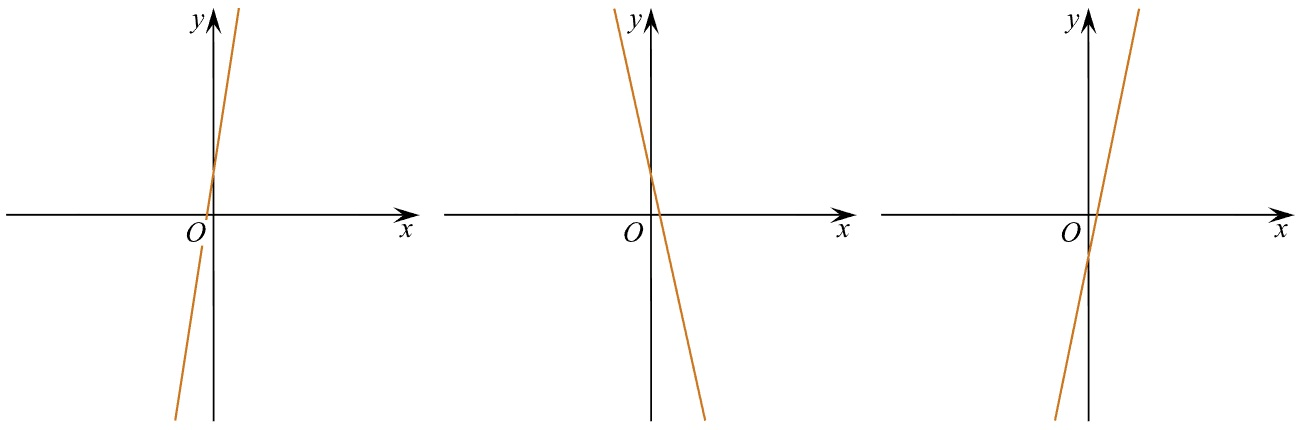
\includegraphics[align=t, width=\linewidth]{\picpath/G71M9L4-3}
		\end{minipage}
		\\
		\\
		\begin{minipage}[t]{\linewidth}
			\begin{tasks}(4)
				\task \( k<0, b>0 \)
				\task \( k>0, b>0 \)
				\task \( k<0, b<0 \)
				\task \( k>0, b<0 \)
			\end{tasks}
		\end{minipage}
		
		\item Прямая \(y=kx+b\) пересекает ось \(x\) в точке \((18; 0)\), а ось \(y\) --- в точке \((0; 9)\). Запишите уравнение этой прямой и постройте график.
		
		
		\item Постройте графики функции:
		\begin{tasks}(4)
			\task \( y=x-5 \)
			\task \( y=-5x+3 \)
			\task \( y=\dfrac{ x }{ 2 }-6 \)
			\task \( y=|x| \)
		\end{tasks}
				%С188-189
		\item Решите системы уравнений:
		\begin{tasks}(2)
			\task \( \begin{cases} 3x+1=0 \\ 2x+y-5=0 \end{cases} \)
			\task \( \begin{cases} 2x-5=0 \\ 3x+2=0 \end{cases} \)
			\task \( \begin{cases} 5x-1=0 \\ 3y+2=0 \end{cases} \)
			\task \( \begin{cases} x+y-3=0 \\ 2x-3y-1=0 \end{cases} \)
			\task \( \begin{cases} x-y+4=0 \\ 3x+4y+5=0 \end{cases} \)
			\task \( \begin{cases} 2x+3y=-1 \\ 3x-2y=0 \end{cases} \)
			\task \( \begin{cases} -x+y=2 \\ -2x-5y=0 \end{cases} \)
			\task \( \begin{cases} -4x-5=5y \\ 3x-11y=5 \end{cases} \)
		\end{tasks}
		
		
	\end{listofex}
\end{class}
%END_FOLD

%BEGIN_FOLD % ====>>_ Домашняя работа 2 _<<====
\begin{homework}[number=2]
	\begin{listofex}
		\item Постройте систему координат и отметьте точки
		\begin{tasks}(4)
			\task \( A(4;3) \)
			\task \( B(2;4) \)
			\task \( C(-5;2) \)
			\task \( D(4;-3) \)
			\task \( E(-5;-1) \)
			\task \( M(1;3) \)
			\task \( N(3;0) \)
			\task \( K(0;4) \)
		\end{tasks}
		\item Постройте графики функции:
		\begin{tasks}(3)
			\task \( y=0,5 \cdot x +5 \)
			\task \( y=-x+4 \)
			\task \( y=-4x+7 \)
		\end{tasks}
		
		\item Решите системы уравнений:
		\begin{tasks}(2)
			\task \( \begin{cases} 2x+4y=-6 \\ -2x-5=2y \end{cases} \)
			\task \( \begin{cases} 5x-1=-y \\ 4x-5y-2=0 \end{cases} \)
			\task \( \begin{cases} -y+6x=-5 \\ 4x+9y=-2 \end{cases} \)
			\task \( \begin{cases} 6y-8x-3 \\ -5x+7y=2 \end{cases} \)
		\end{tasks}
		%\item Решите системы уравнений:
		%\begin{tasks}
		%	\task \( \begin{cases}  \\  \end{cases} \)
		%	\task \( \begin{cases}  \\  \end{cases} \)
		%	\task \( \begin{cases}  \\  \end{cases} \)
		%	\task \( \begin{cases}  \\  \end{cases} \)
		%\end{tasks}
	\end{listofex}
\end{homework}
%END_FOLD

%BEGIN_FOLD % ====>>_____ Занятие 5 _____<<====
\begin{class}[number=5]
	\begin{listofex}
		%BANK https://math-oge.sdamgia.ru/test?likes=341325
		%341702
		\item На рисунке изображены графики функций вида \(y = kx + b\). Установите соответствие между графиками функций и знаками коэффициентов \(k\) и \(b\).
		\begin{minipage}[t]{\linewidth}
			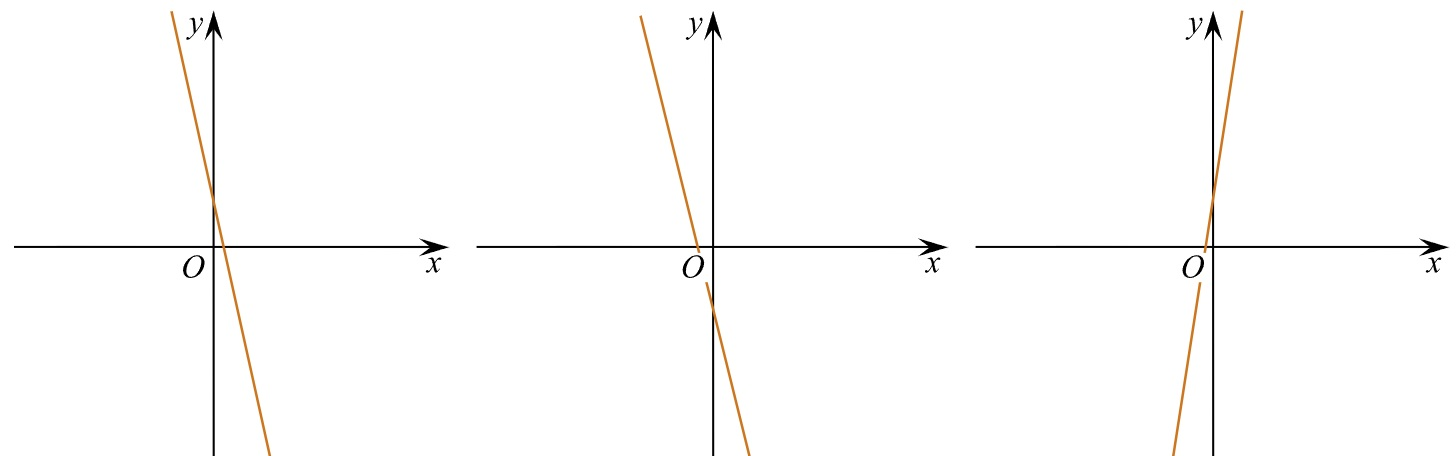
\includegraphics[align=t, width=\linewidth]{\picpath/G71M9L5-1}
		\end{minipage}
		\\
		\\
		\begin{minipage}[t]{\linewidth}
			\begin{tasks}(3)
				\task \( k<0, b>0 \)
				\task \( k>0, b>0 \)
				\task \( k<0, b<0 \)
			\end{tasks}
		\end{minipage}
		\item Определите в каких четвертях координатной плоскости лежит график функции и постройте его:
		\begin{tasks}(4)
			\task \( y=x \)
			\task \( y=x-5 \)
			\task \( y=2x \)
			\task \( y=4 \)
			\task \( y=8-x \)
			\task \( y=-x+6 \)
			\task \( y=-3x+2 \)
			\task \( y=0,5x-7 \)
		\end{tasks}
		\item Прямая \(y=kx+b\) пересекает ось \(x\) в точке \((12; 0)\), а ось \(y\) --- в точке \((0; -6)\). Запишите уравнение этой прямой и постройте график.
		%265
		\item Задайте формулой линейную функцию, график которой параллелен прямой \(y=5-2x\) и проходит через точку \(A(2; 7)\).
		\item Решите системы уравнений:
		\begin{tasks}(2)
			\task \( \begin{cases} y-x=9 \\ 2x+y=-2 \end{cases} \)
			\task \( \begin{cases} 2x-3y=7 \\ 3-y=5x \end{cases} \)
			\task \( \begin{cases} 0,5x+6-y=0 \\ 2x-3y=1 \end{cases} \)
			\task \( \begin{cases} \dfrac{ y }{ 2 }-5x=11 \\ 3x-2+y=0 \end{cases} \)
			\task \( \begin{cases} 4y-x=0,25 \\ 1,5x=3y-2 \end{cases} \)
			\task \( \begin{cases} 7x-3y+5=0 \\ 3x-7y=4 \end{cases} \)
		\end{tasks}
	\end{listofex}
\end{class}
%END_FOLD

%BEGIN_FOLD % ====>>_____ Занятие 6 _____<<====
\begin{class}[number=6]
	\begin{listofex}
		\item Занятие 6
	\end{listofex}
\end{class}
%END_FOLD

%BEGIN_FOLD % ====>>_ Домашняя работа 3 _<<====
\begin{homework}[number=3]
	\begin{listofex}
		\item На рисунке изображены графики функций вида \(y = kx + b\). Установите соответствие между графиками функций и знаками коэффициентов \(k\) и \(b\).
		\begin{minipage}[t]{\linewidth}
			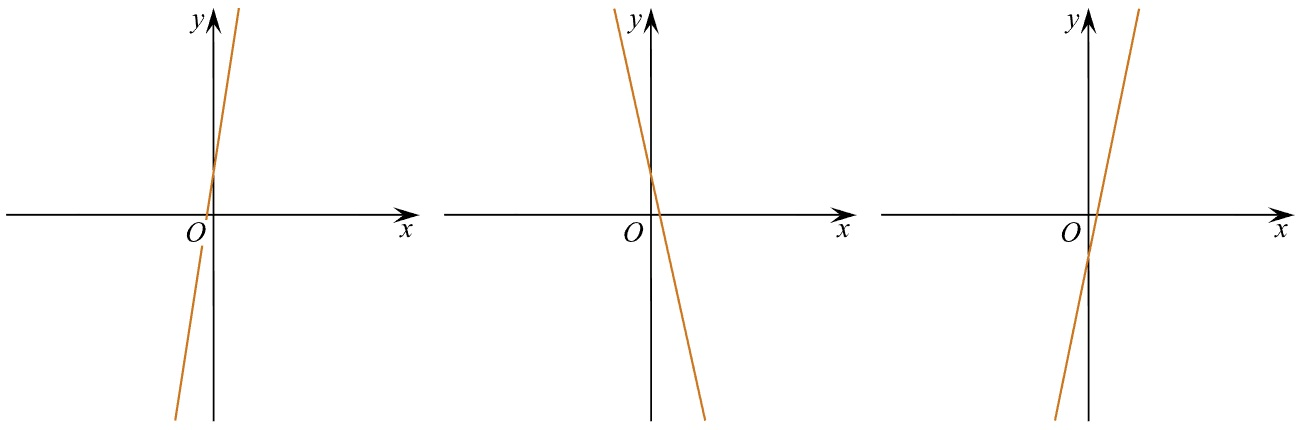
\includegraphics[align=t, width=\linewidth]{\picpath/G71M9L4-3}
		\end{minipage}
		\\
		\\
		\begin{minipage}[t]{\linewidth}
			\begin{tasks}(4)
				\task \( k<0, b>0 \)
				\task \( k>0, b>0 \)
				\task \( k<0, b<0 \)
				\task \( k>0, b<0 \)
			\end{tasks}
		\end{minipage}
		%266-267
		\item Задайте формулой линейную функцию, график которой параллелен прямой \(y=-2x+5\) и проходит через точку \( A(1; 5) \).
		\item Задайте формулой линейную функцию, график которой параллелен прямой \(y=2x+3\) и проходит через точку \( B(1; 2) \).
		\item Решите системы уравнений:
		\begin{tasks}(3)
			\task \( \begin{cases} 5y-4x=11 \\ x-8y=5 \end{cases} \)
			\task \( \begin{cases} 8-3x=-6y \\ 15y-2x=7 \end{cases} \)
			\task \( \begin{cases} -5x+2=3y \\ -4x=7y-3 \end{cases} \)
		\end{tasks}
	\end{listofex}
\end{homework}
%END_FOLD

%BEGIN_FOLD % ====>>_____ Занятие 7 _____<<====
\begin{class}[number=7]
	\begin{listofex}
		\item Определите в каких четвертях координатной плоскости лежит график функции и постройте его:
		\begin{tasks}(4)
			\task \( y=-2x \)
			\task \( y=3-x \)
			\task \( y=-\dfrac{ x }{ 2 }+7 \)
			\task \( y=-2x+4 \)
			\task \( y=-x-4 \)
			\task \( y=4x+1 \)
			\task \( y=-\dfrac{ 3x }{ 4 }+6 \)
			\task \( y=0,25x-8 \)
		\end{tasks}
		\item Задайте формулой линейную функцию, график которой параллелен прямой \(y=6+2x\) и проходит через точку \(A(7; -12)\).
		\item Задайте формулой линейную функцию, график которой параллелен прямой \(y=-4-x\) и проходит через точку \(A(12; -8)\).
		\item Решите системы уравнений:
		\begin{tasks}(2)
			\task \( \begin{cases} y+2x=-3 \\ 4x-y=2 \end{cases} \)
			\task \( \begin{cases} 3x-5y=7 \\ 7-y=2x \end{cases} \)
			\task \( \begin{cases} 4x-5y-3=0 \\ 5x-6y=1 \end{cases} \)
			\task \( \begin{cases} -2x-3y=2 \\ 2x+6=-y \end{cases} \)
			\task \( \begin{cases} -x+3=-6y \\ 10x-9=3y \end{cases} \)
			\task \( \begin{cases} 3y-5x=2 \\ -5+x=-3y \end{cases} \)
		\end{tasks}
		\item Разность двух чисел равна \(13\), а их удвоенная сумма равна \(54\). Найдите числа.
		%\item Сумма двух чисел равна \(21\), а их разность равна \(9\). Найдите числа.
		\item Одно число в \(2\) раза больше другого. Если меньшее из этих чисел увеличить в \(4\) раза, а большее увеличить в \(2\) раза, то их сумма будет равна \(44\). Найдите числа.
		\item В прямоугольнике, периметр которого равен \(52\) см, разность длин двух сторон равна \(4\) см. Найдите стороны прямоугольника.
		\item Для класса, в котором учатся \(30\) учеников, купили билеты в театр стоимостью по \(100\) и \(150\) р. Сколько было куплено отдельно тех и других билетов, если их общая стоимость составила \(3500\) р.?
		%\item Школьники поехали на экскурсию. Обратно они возвращались другим путем, который был на \(7\) км короче первого. Какова длина каждого пути, если всего в оба конца школьники проехали \(41\) км.
	\end{listofex}
\end{class}
%END_FOLD

%BEGIN_FOLD % ====>>_ Проверочная работа _<<====
\begin{class}[number=8]
	\begin{listofex}
		\item Постройте графики функций:
		\begin{tasks}(2)
			\task \( y=-4x+5 \)
			\task \( y=0,5x-11 \)
			\task \( y=4x+7 \)
			\task \( y=-\dfrac{ x }{ 3 }-6 \)
		\end{tasks}
		\item Задайте формулой линейную функцию, график которой параллелен прямой \(y=6+2x\) и проходит через точку \(A(7; -12)\).
		\item Задайте формулой линейную функцию, график которой параллелен прямой \(y=-4-x\) и проходит через точку \(A(12; -8)\).
		\item Решите системы уравнений:
		\begin{tasks}(2)
			\task \( \begin{cases} x+2y=-4 \\ 2x=y-5 \end{cases} \)
			\task \( \begin{cases} 5x-2y=3 \\ 3-4y=3x \end{cases} \)
			\task \( \begin{cases} 2y+3x=2\\-3x-4x=8 \end{cases} \)
			\task \( \begin{cases} 5y-6x=-7 \\ -6y-2x=8 \end{cases} \)
			%\task \( \begin{cases} \\ \end{cases} \)
			%\task \( \begin{cases} \\ \end{cases} \)
		\end{tasks}
		
		\item Одно число в \(2\) раза больше другого. Если меньшее из этих чисел увеличить в \(4\) раза, а большее увеличить в \(2\) раза, то их сумма будет равна \(44\). Найдите числа.
		\item В прямоугольнике, периметр которого равен \(52\) см, разность длин двух сторон равна \(4\) см. Найдите стороны прямоугольника.
		\item Для класса, в котором учатся \(30\) учеников, купили билеты в театр стоимостью по \(100\) и \(150\) р. Сколько было куплено отдельно тех и других билетов, если их общая стоимость составила \(3500\) р.?
		\item Рассчитываясь за покупку, мальчик получил сдачи \(70\) рублей монетами достоинством \(5\) и \(10\) рублей. Всего он получил \(10\) монет. Сколько монет достоинством \(5\) рублей он получил?
		%\item Школьники поехали на экскурсию. Обратно они возвращались другим путем, который был на \(7\) км короче первого. Какова длина каждого пути, если всего в оба конца школьники проехали \(41\) км.
	\end{listofex}
\end{class}
%END_FOLD

%BEGIN_FOLD % ====>>_ Проверочная работа _<<====
\begin{class}[number=9]
	\begin{listofex}
		\item Задайте формулой линейную функцию, график которой параллелен прямой \(y=3+x\) и проходит через точку \(A(5; 2)\).
		\item Задайте формулой линейную функцию, график которой параллелен прямой \(y=-5+2x\) и проходит через точку \(A(6; -8)\).
		\item Задайте формулой линейную функцию, график которой параллелен прямой \(y=5-2x\) и проходит через точку \(A(2; 7)\).
		\item Прямая \(y=kx+b\) пересекает ось \(x\) в точке \((18; 0)\), а ось \(y\) --- в точке \((0; 9)\). Запишите уравнение этой прямой и постройте график.
		
		
		\item Одно число в \(2\) раза больше другого. Если меньшее из этих чисел увеличить в \(4\) раза, а большее увеличить в \(2\) раза, то их сумма будет равна \(44\). Найдите числа.
		\item В прямоугольнике, периметр которого равен \(52\) см, разность длин двух сторон равна \(4\) см. Найдите стороны прямоугольника.
		\item Для класса, в котором учатся \(30\) учеников, купили билеты в театр стоимостью по \(100\) и \(150\) р. Сколько было куплено отдельно тех и других билетов, если их общая стоимость составила \(3500\) р.?
		\item Рассчитываясь за покупку, мальчик получил сдачи \(70\) рублей монетами достоинством \(5\) и \(10\) рублей. Всего он получил \(10\) монет. Сколько монет достоинством \(5\) рублей он получил?
		%\item Школьники поехали на экскурсию. Обратно они возвращались другим путем, который был на \(7\) км короче первого. Какова длина каждого пути, если всего в оба конца школьники проехали \(41\) км.
		\item Решите системы уравнений:
		\begin{tasks}(2)
			\task \( \begin{cases} 2y+3x=2\\-3x-4x=8 \end{cases} \)
			\task \( \begin{cases} 5y-6x=-7 \\ -6y-2x=8 \end{cases} \)
			%\task \( \begin{cases} \\ \end{cases} \)
			%\task \( \begin{cases} \\ \end{cases} \)
		\end{tasks}
	\end{listofex}
\end{class}
%END_FOLD